\documentclass[12pt]{article}

\usepackage{graphicx}% Include figure files
\usepackage{dcolumn}% Align table columns on decimal point

% Use Arial font %
\usepackage{helvet}
\renewcommand{\familydefault}{\sfdefault} 

% Default margins and paper properties %
\usepackage[a4, portrait, margin=0.6in]{geometry}

\begin{document}
	\title{Hypothesis plots summary} % Force line breaks with \\
	\author{1666957, Gustavo Espinal Lugo}
	\date{\today} % It is always \today, today, %  but any date may be explicitly specified

	\maketitle
	%\tableofcontents
	
	\section*{Plots and corresponding metadata}
	mean expected W mass: 80.379 $[GeV/c^{2}]$,\\
mean hypothesis masses: [78.  78.5 79.  79.5 80.  80.5 81.  81.5 82. ] $[GeV/c^{2}]$,\\
mass width: 2.07 $[GeV/c^{2}]$,\\
chi\_square value of hypothesis fit: 1.5415639895735953\\
	Absolute path to figure: /home/physics/phuxdp/Desktop/PX402 Physics Project/WBosonProject/T2W5/plots/muPT\_80.379\_2.07\_between\_78\_and\_82\_summary.png\\
	Next lines are the data of the shown histograms (if needed): \\
	All quantities: 	80.379, [78.  78.5 79.  79.5 80.  80.5 81.  81.5 82. ], 2070, 1.5415639895735953\\
	X\_energ\_vls = [0.6, 1.7999999999999998, 3.0, 4.199999999999999, 5.4, 6.6, 7.8, 9.0, 10.2, 11.399999999999999, 12.6, 13.799999999999999, 15.0, 16.2, 17.4, 18.6, 19.799999999999997, 21.0, 22.2, 23.4, 24.6, 25.799999999999997, 27.0, 28.199999999999996, 29.4, 30.6, 31.799999999999997, 33.0, 34.2, 35.4, 36.599999999999994, 37.8, 39.0, 40.2, 41.4, 42.599999999999994, 43.8, 45.0, 46.2, 47.4, 48.599999999999994, 49.8, 51.0, 52.2, 53.4, 54.599999999999994, 55.8, 57.0, 58.199999999999996, 59.4, 60.599999999999994, 61.8, 63.0, 64.19999999999999, 65.4, 66.6, 67.8, 69.0, 70.19999999999999, 71.4, 72.6, 73.8, 75.0, 76.19999999999999, 77.4, 78.6, 79.8, 81.0, 82.19999999999999, 83.4, 84.6, 85.8, 87.0, 88.19999999999999, 89.4, 90.6, 91.8, 93.0, 94.19999999999999, 95.4, 96.6, 97.8, 99.0, 100.19999999999999, 101.4, 102.6, 103.8, 105.0, 106.19999999999999, 107.4, 108.6, 109.8, 111.0, 112.19999999999999, 113.4, 114.6, 115.79999999999998, 117.0, 118.19999999999999, 119.4]\\
	Y\_data\_bin\_cnts = [0.0, 0.0, 0.0, 0.0, 0.0, 0.0, 0.0, 0.0, 0.0, 0.0, 0.0, 0.0, 0.0, 0.0, 0.0, 0.0, 0.0, 0.0, 8.0, 415.0, 524.0, 546.0, 600.0, 611.0, 609.0, 614.0, 637.0, 656.0, 678.0, 667.0, 607.0, 610.0, 543.0, 405.0, 337.0, 251.0, 185.0, 166.0, 116.0, 108.0, 93.0, 69.0, 50.0, 67.0, 46.0, 47.0, 27.0, 25.0, 23.0, 28.0, 19.0, 22.0, 24.0, 26.0, 14.0, 19.0, 10.0, 9.0, 6.0, 7.0, 9.0, 9.0, 11.0, 8.0, 5.0, 10.0, 5.0, 3.0, 6.0, 4.0, 2.0, 3.0, 4.0, 4.0, 3.0, 2.0, 3.0, 1.0, 1.0, 3.0, 0.0, 4.0, 1.0, 1.0, 1.0, 1.0, 2.0, 0.0, 0.0, 1.0, 0.0, 1.0, 1.0, 0.0, 0.0, 0.0, 0.0, 1.0, 2.0, 0.0]\\
	Y\_model\_bin\_cnts = [0.0, 0.0, 0.0, 0.0, 0.0, 0.0, 0.0, 0.0, 0.0, 0.0, 0.0, 0.0, 0.0, 0.0, 0.0, 0.0, 0.0, 0.0, 8.647396087646484, 395.85760498046875, 480.4093322753906, 527.4892578125, 553.4312744140625, 568.8042602539062, 571.686767578125, 607.2369995117188, 660.0816650390625, 686.0238037109375, 632.218017578125, 611.0799560546875, 591.86376953125, 560.15673828125, 483.2912902832031, 417.9559326171875, 315.14862060546875, 238.28334045410156, 199.85061645507812, 157.57469177246094, 147.966552734375, 98.00386810302734, 94.1605453491211, 64.37507629394531, 63.41425704956055, 53.80601501464844, 34.5895881652832, 41.31534194946289, 43.237003326416016, 24.981374740600586, 36.51123809814453, 24.981365203857422, 23.05971908569336, 18.255619049072266, 21.138080596923828, 19.216461181640625, 16.333972930908203, 15.373154640197754, 12.49068546295166, 8.647391319274902, 5.764925479888916, 4.804107666015625, 5.764931678771973, 10.569037437438965, 6.72574520111084, 3.843287229537964, 9.608217239379883, 5.764933109283447, 6.725752830505371, 6.7257537841796875, 4.804112434387207, 2.882465362548828, 5.764929294586182, 2.8824663162231445, 2.8824565410614014, 0.0, 2.8824644088745117, 2.8824639320373535, 0.9608219265937805, 6.725756645202637, 2.8824687004089355, 1.9216444492340088, 1.9216464757919312, 0.9608224630355835, 0.9608215093612671, 0.9608214497566223, 0.9608220458030701, 1.9216439723968506, 0.9608096480369568, 0.0, 1.9216431379318237, 0.0, 0.960809588432312, 0.0, 1.921645998954773, 1.921644926071167, 0.0, 0.9608221650123596, 2.8824658393859863, 0.0, 0.9608216285705566, 0.0]\\

    Found optimal massses ($\chi^2$ roots): [81.04356316] $[GeV/c^{2}]$
    Uncertainty [GeV/c^2]: 1.4210854715202004e-14

	\begin{figure}[tb]
		\centering
		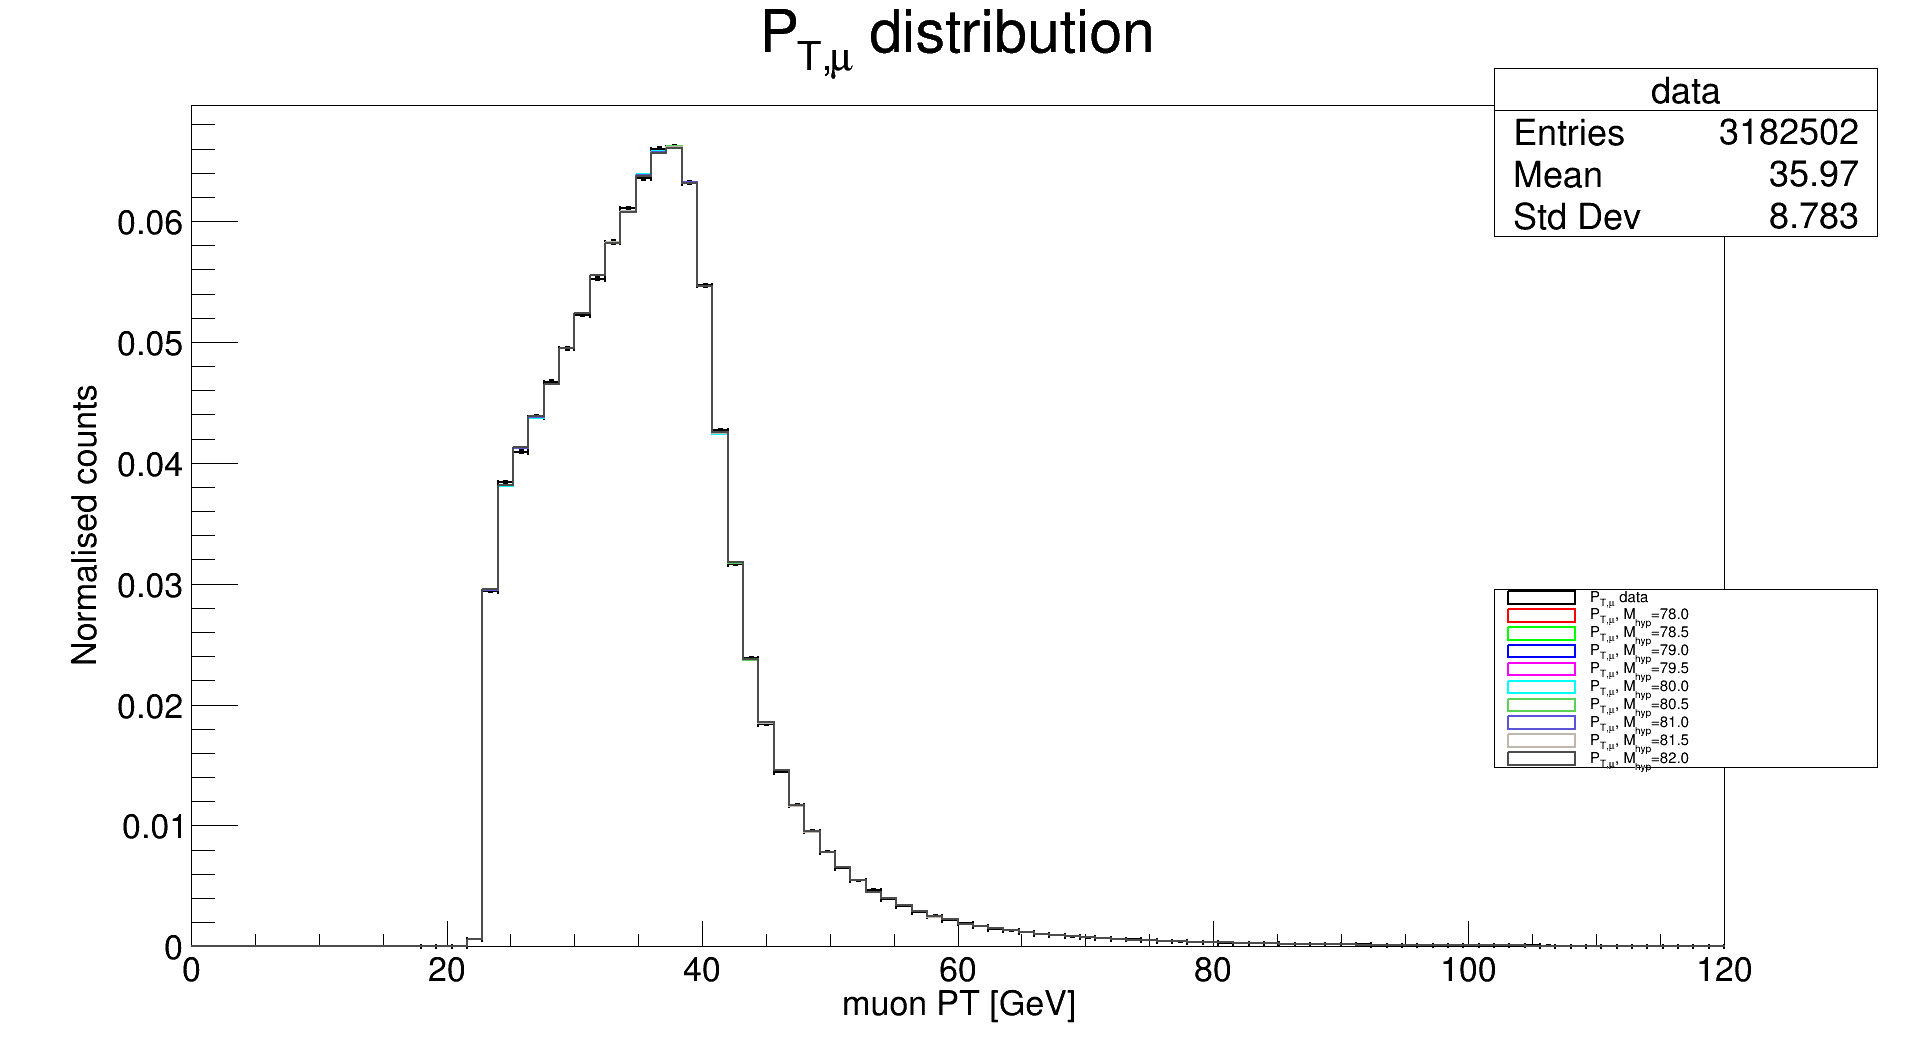
\includegraphics[width=\columnwidth]{/home/physics/phuxdp/Desktop/PX402 Physics Project/WBosonProject/T2W5/plots/muPT_80.379_2.07_between_78_and_82_summary.png}
		\caption{\small Hypothesis masses mean expected W mass: 80.379 $[GeV/c^{2}]$,\\
mean hypothesis masses: [78.  78.5 79.  79.5 80.  80.5 81.  81.5 82. ] $[GeV/c^{2}]$,\\
mass width: 2.07 $[GeV/c^{2}]$,\\
chi_square value of hypothesis fit: 1.5415639895735953. }
		\label{fig: fig_0}
	\end{figure}

       \begin{figure}[tb]
		\centering
		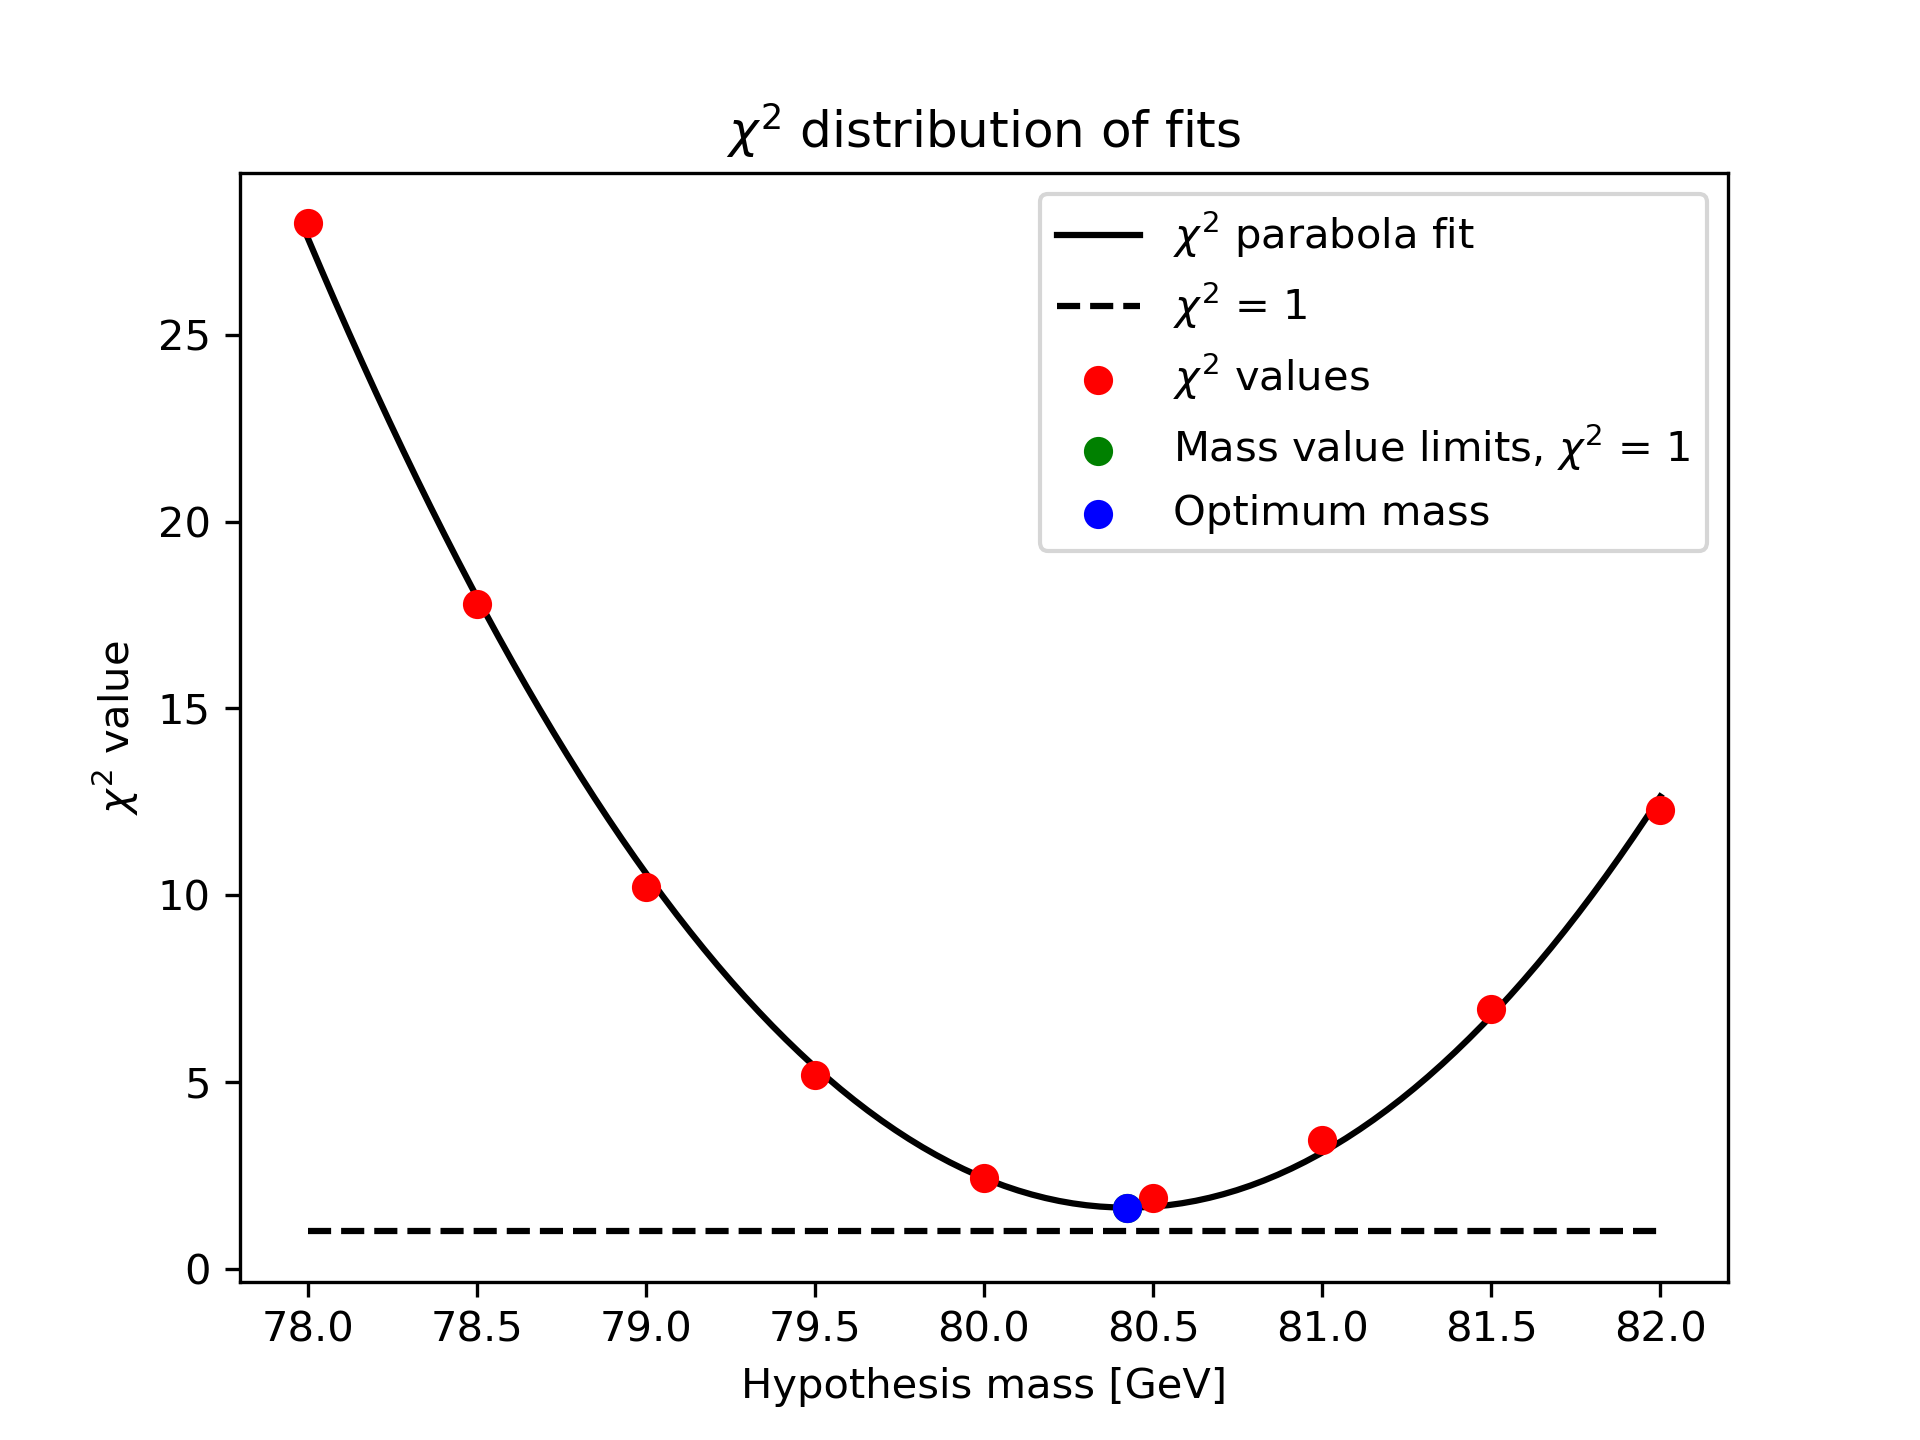
\includegraphics[width=\columnwidth]{/home/physics/phuxdp/Desktop/PX402 Physics Project/WBosonProject/T2W5/plots/chi_square_fits_muPT_80.379_2.07_between_78_and_82_summary.png}
		\caption{\small $\chi^2$ of hypothesis masses. }
		\label{fig: fig_chi_square}
	\end{figure}

    \begin{figure}[tb]
		\centering
		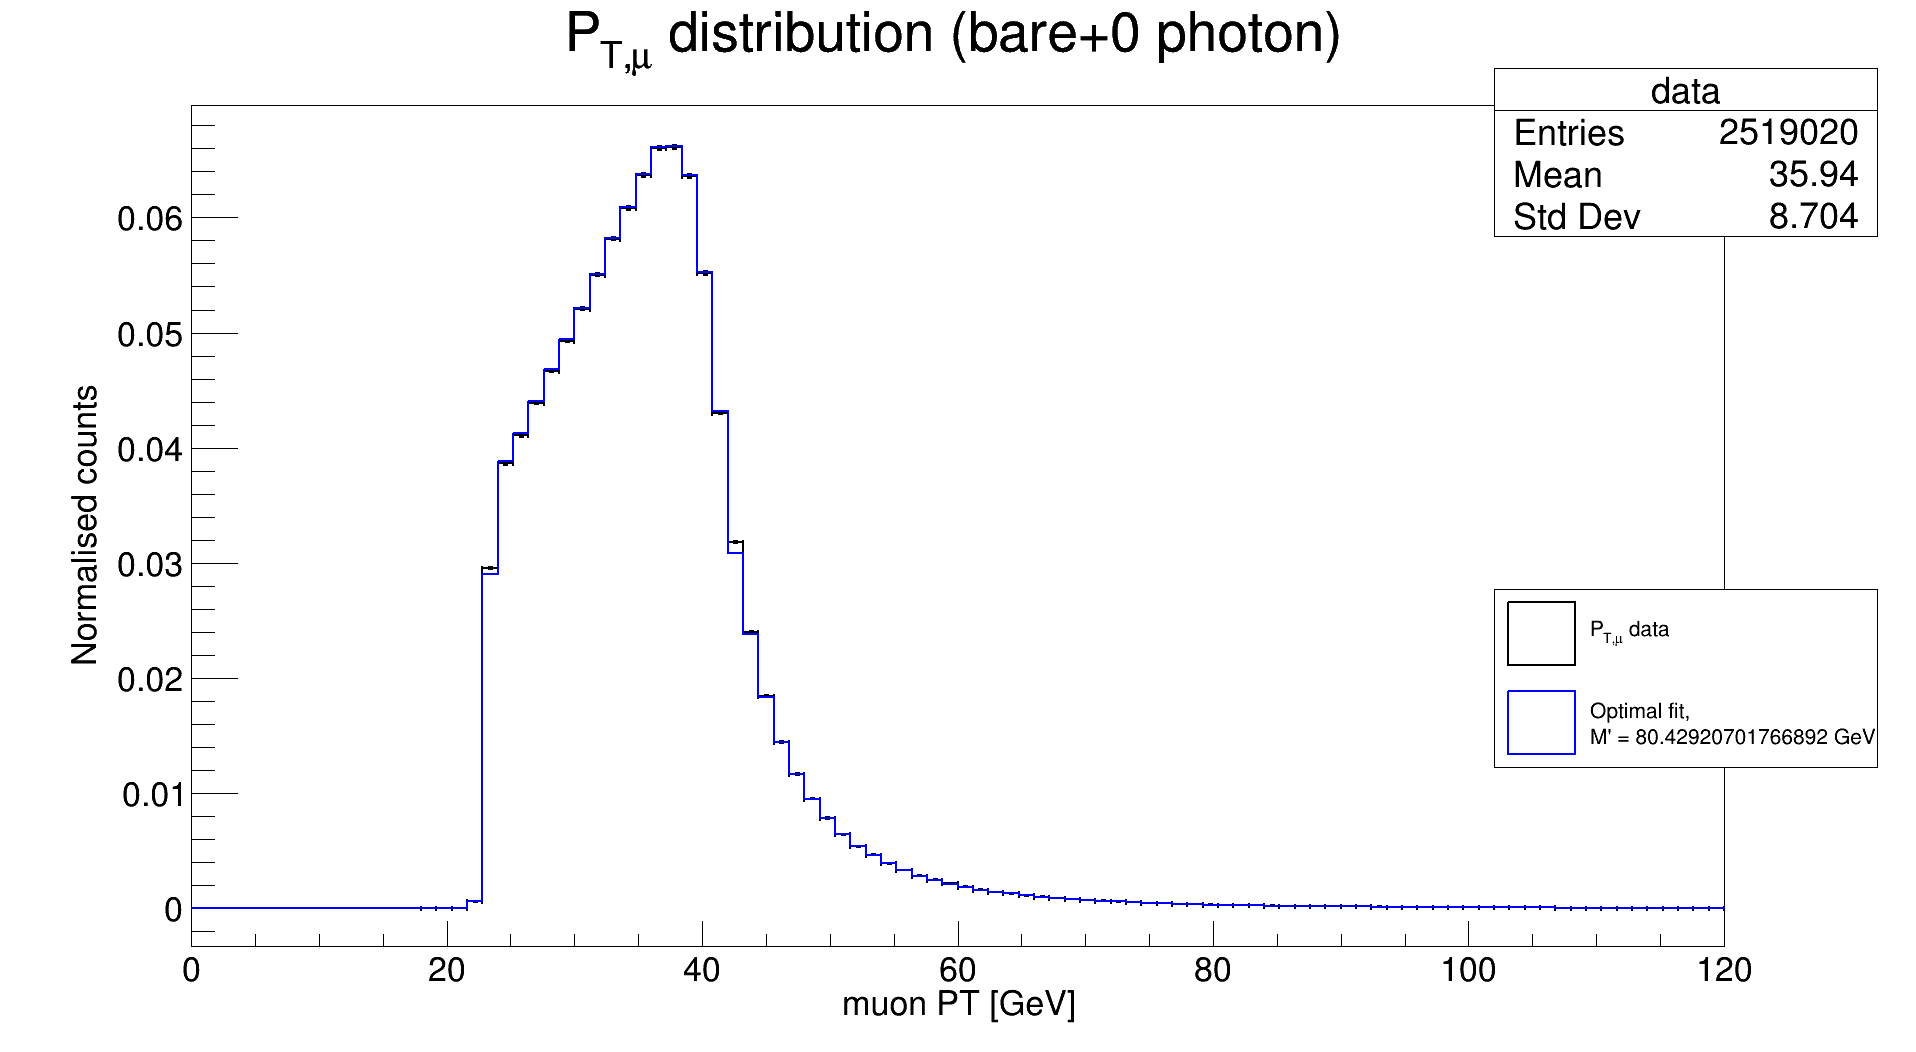
\includegraphics[width=\columnwidth]{/home/physics/phuxdp/Desktop/PX402 Physics Project/WBosonProject/T2W5/plots/optimum_muPT_80.379_2.07_between_78_and_82_summary.png}
		\caption{\small Data and optimum fit with $\chi^2 = 0.029311644621615302$. Used the hypothesis mass of 81.04356316417679$\pm$1.4210854715202004e-14 $[GeV/c^{2}]$. }
		\label{fig: fig_optim_parms}
	\end{figure}
    
\end{document}